% Intestazione
\fancyhead[L]{4 \hspace{0.2cm} Guida all’utilizzo} % Testo a sinistra 

\section{Guida all’utilizzo}
\label{sec:guida_utilizzo}
% Screenshot di cosa appare all'avvio del chatbot. Descrivere gli elementi presenti nella schermata iniziale.


\subsection{Cosa chiedere, e come chiederlo}
\label{subsec:cosa_come_chiedere}

BuddyBot è pensato per essere l'assistente digitale di un'azienda informatica che desidera aiutare i propri dipendenti a ricercare in
modo veloce le informazioni di interesse nel codice e nella documentazione dei vari progetti aziendali. Più precisamente, ad
ogni interrogazione posta dall'utente vengono associati
dei documenti di contesto, che provengono esclusivamente dai profili \emph{GitHub}\textsubscript{\textbf{\textit{G}}},
\emph{Jira}\textsubscript{\textbf{\textit{G}}} e \emph{Confluence}\textsubscript{\textbf{\textit{G}}} dell'azienda, e, in base alle
informazioni presenti su tali documenti di contesto, il chatbot fornirà la risposta alla domanda ricevuta.
Se la domanda viene malposta, il chatbot potrebbe non essere in grado di fornire una risposta, e in tal caso potrebbe restituire
uno dei seguenti messaggi:
\begin{itemize}
    \item \emph{"Domanda fuori contesto"}: la domanda posta non è inerente al contesto informatico aziendale;
    \item \emph{"Informazione non trovata"}: non è stato possibile trovare nei documenti di contesto informazioni utili per rispondere
    alla domanda.
\end{itemize}

E' tuttavia possibile che il chatbot restituisca tali risposte anche in casi in cui non ce lo si aspetta.
Per evitare di ottenere risposte negative, forniamo qui di seguito delle istruzioni per capire come porre la domanda per
ottenere una risposta soddisfacente:
\begin{itemize}
    \item La domanda deve essere concisa e diretta, senza giri di parole. Ad esempio "Qual è lo stato del progetto X su Jira?" invece
    che "Potresti gentilmente dirmi qual è lo stato attuale del progetto X su Jira, per favore?";
    \item Si devono mettere bene in risalto le parole chiave. Ad esempio "Qual è l'errore di build nel progetto Y?" invece che "Qual
    è il problema con il progetto Y?";
    \item La domanda deve essere il più breve possibile. Ad esempio "Chi è l'assegnatario del ticket Z?" invece che "Vorrei sapere
    chi è la persona a cui è stato assegnato il ticket Z";
    \item La domanda deve essere pensata per ottenere una risposta unitaria, e non per aprire una discussione. Ad esempio, occorre
    unificare "Quali commit sono stati fatti oggi? Mostrameli in forma di tabella con assegnatario e data" invece che porre due domande
    separate "Quali commit sono stati fatti oggi?" e "Mostrameli in forma di tabella con assegnatario e data", perchè in quest'ultimo
    caso la seconda domanda riceverà come risposta "Domanda fuori contesto": infatti, ogni coppia domanda-risposta è a sè stante, cioè
    il chatbot non considera il completo flusso del discorso per generare la risposta all'interrogazione corrente, bensì considera solo
    quest'ultima. Le domande suggerite per proseguire sono infatti pensate per guidare l'utente verso una nuova interrogazione, e non per far
    completare la risposta alla domanda corrente;
    \item La domanda deve riguardare un contesto chiaro e definito, quindi non può toccare tematiche troppo generali. Ad esempio
    "Quali sono i task aperti per il progetto A?" invece che "Qual è la situazione dei nostri progetti?";
    \item Il suddetto contesto deve essere uno, infatti non si possono porre due o più domande a tema differente in una stessa
    interrogazione. Ad esempio, invece che "Chi è l'assegnatario del ticket Z su Jira
    e quali sono i suoi relativi commit su GitHub?", è meglio separare in "Chi è l'assegnatario del ticket Z su Jira?" e poi, una 
    volta ricevuta la risposta, "Quali sono i commit di persona Y su GitHub?" (specificando chiaramente la persona, poichè, come suddetto, il chatbot non può visualizzare il messaggio precedente);
    \item Non si devono chiedere informazioni generiche a riguardo di una risorsa fornendo solo il nome della stessa, ma bisogna
    bensì specificare più di preciso cosa si vuole sapere a riguardo di tale risorsa. Ad esempio "Qual è la descrizione del ticket
    Z su Jira?" invece che "Dimmi qualcosa sul ticket Z";
    \item La domanda deve essere posta in un linguaggio quanto più possibile formale e tecnico, cercando di rimanere aderenti
    allo stile di scrittura dei documenti aziendali. Un linguaggio troppo colloquiale quasi sicuramente condurrà a risposte negative.
    Ad esempio "Qual è la copertura dei test per il modulo B?" invece che "Come stanno andando i test per il modulo B?";
    \item Non si devono porre domande che richiedono una risposta soggettiva. In caso ne venga posta una per sbaglio, non ci si deve
    fidare della risposta fornita, è bensì consigliabile chiedere ad un collega. Ad esempio "A quanto ammonta la copertura del codice
    nel progetto C?" invece che "Pensi che il codice del progetto C sia buono?";
    \item Si devono evitare domande che richiedano ragionamento e/o collegamenti logici, in quanto il chatbot non è in grado di
    processare informazioni in tal senso. Ad esempio "Quali sono i commit svolti tra il 6 ed il 10 febbraio nel progetto D?" invece che "Quali sono i
    commit nel progetto D dall'inizio della sprint ad ora?";
    \item Non si devono porre domande per la cui risposta è necessaria una ricerca su internet, in quanto il chatbot fa
    riferimento esclusivamente ai documenti di contesto, e non è in grado di navigare in rete. Ad esempio, invece che "Nel
    progetto Y viene utilizzata l'ultima versione rilasciata del framework X?", bisogna chiedere "Qual è la versione del framework X
    che viene utilizzata nel progetto Y?" e poi cercare manualmente su internet se tale versione è l'ultima rilasciata o meno.
\end{itemize}


\subsection{Interrogazione del chatbot}

\subsubsection{Come inserire una domanda}
% Parlare dei due metodi di inserimento, o domanda libera o (dalla seconda domanda in poi) selezione di una delle domande per
% proseguire la conversazione.

\subsubsection{La risposta del chatbot}
% Parlare:
% - della risposta testuale (che può contenere uno snippet di codice in un apposito riquadro);
% - della possibilità di copiare il testo, e soprattutto di copiare lo snippet di codice, entrambi mediante pulsante apposito;
% - della visualizzazione dei link correlati nell'apposito riquadro.


\subsection{Visualizzazione dello storico dei messaggi}
% Parlare:
% - della vista iniziale (senza messaggi);
% - della visualizzazione della data e ora di invio del messaggio;
% - dello scorrimento verso l'alto per visualizzare i messaggi precedenti fino all'inizio della conversazione;
% - della vista del segnalino "Inizio della conversazione" quando si è raggiunto l'inizio della conversazione.


\subsection{Aggiornamento automatico dei documenti}
Al fine di garantire che le informazioni fornite dal chatbot siano il più possibile attendibili, i documenti di contesto utilizzati per generare le risposte vengono aggiornati ogni 24 ore.
Tali aggiornamenti sono svolti in modo automatico, e non è dunque necessario alcun intervento di configurazione.
È possibile che, nel momento in cui si pone una domanda, l'aggiornamento automatico dei documenti sia in corso, e quindi potrebbe avvenire un errore nella generazione della risposta. In tal caso, è consigliabile attendere qualche minuto e riprovare.
In alto a destra è presente un badge di segnalazione che indica l'esito dell'ultimo aggiornamento:
\begin{itemize}
    \item Se il badge presenta una spunta verde con accanto la scritta \emph{Aggiornato}, significa che l'ultimo aggiornamento è avvenuto con successo, e le risposte fornite
    dal chatbot sono aggiornate ai documenti non più vecchi di 24 ore;
    \item Se il badge presenta una X rossa con accanto la scritta \emph{Non aggiornato}, significa che l'ultimo aggiornamento è fallito, e le risposte fornite dal chatbot potrebbero
    non essere aggiornate ai documenti più recenti;
    \item Se il badge presenta un segnale di pericolo con accanto la scritta \emph{Errore}, significa che non è stato possibile recuperare l'esito dell'ultimo aggiornamento, e
    dunque, non è possibile sapere se le risposte fornite dal chatbot sono aggiornate ai documenti più recenti o meno.
\end{itemize}

\newpage

\begin{figure}[h]
    \centering
        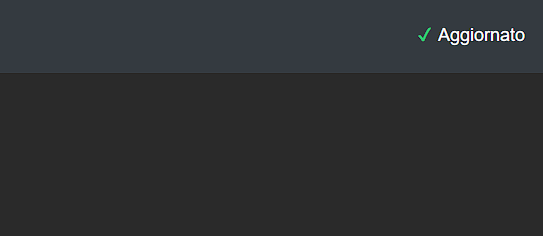
\includegraphics[width=.8\linewidth]{Badge - Aggiornamento avvenuto con successo.png}
        \caption{Badge di aggiornamento avvenuto con successo}
        \label{fig:Aggiornamento avvenuto con successo}        
\end{figure}

\begin{figure}[h]
    \centering
        
\includegraphics[width=.8\linewidth]{Badge - Aggiornamento fallito.png}
        \caption{Badge di aggiornamento fallito}
        \label{fig:Aggiornamento fallito}
\end{figure}

\begin{figure}[h]
    \centering
        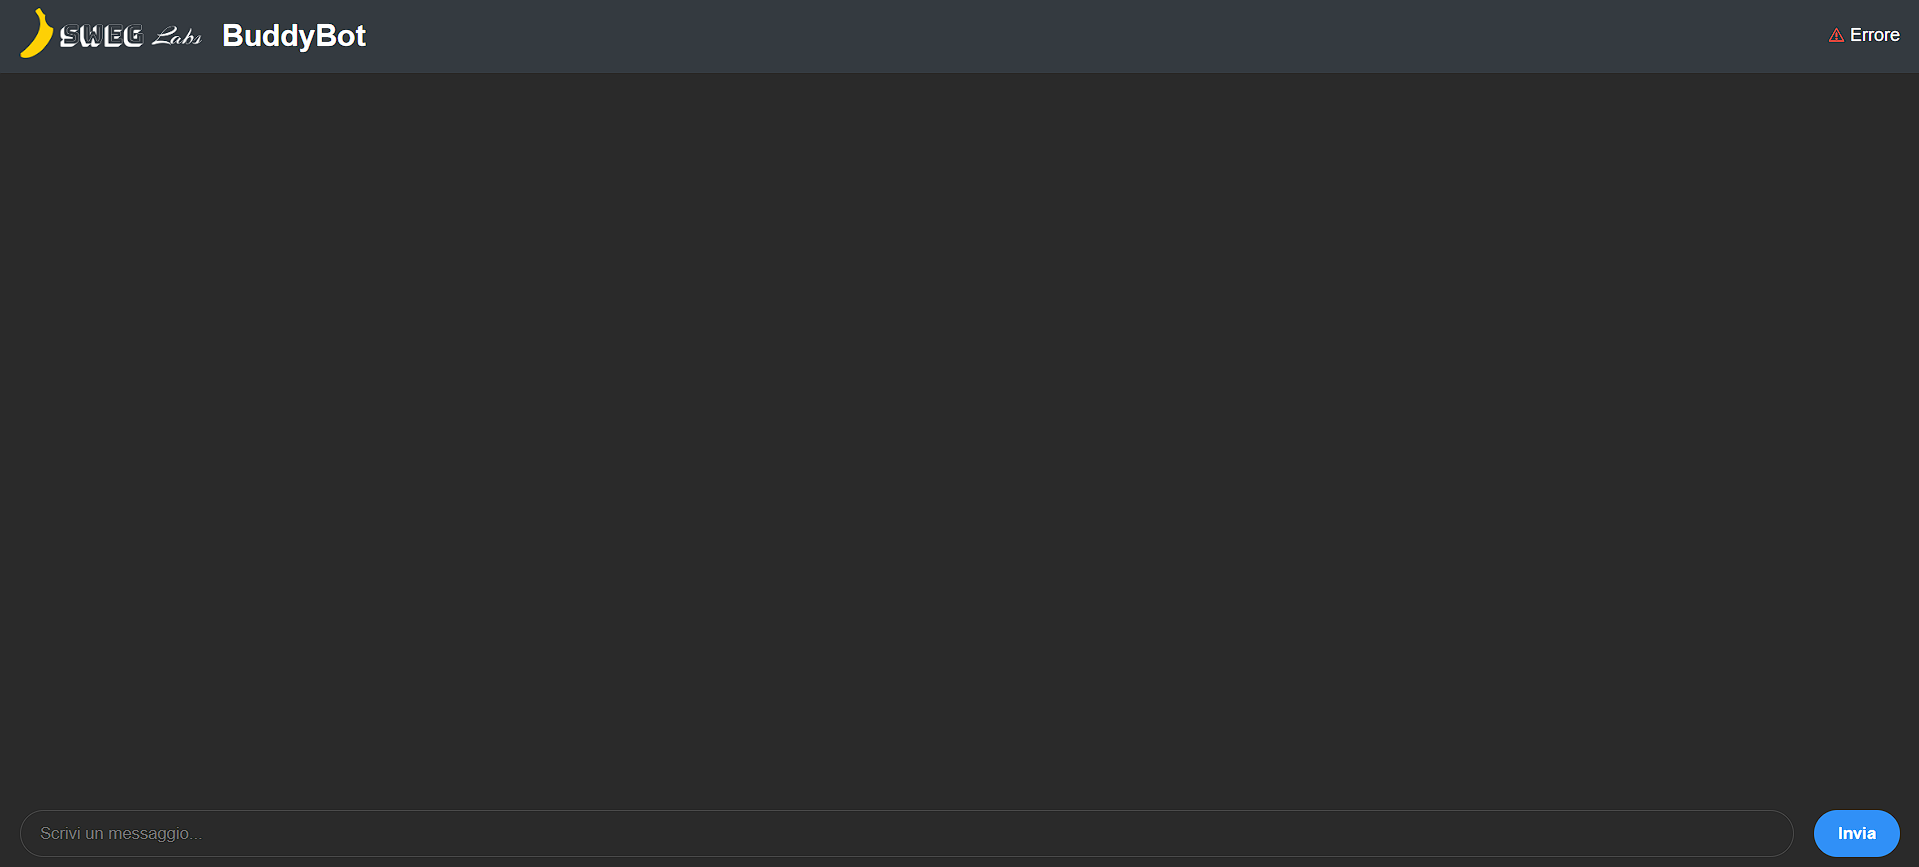
\includegraphics[width=.8\linewidth]{Badge - Errore recupero esito aggiornamento.png}
        \caption{Badge di errore nel recupero dell'esito dell'ultimo aggiornamento}
        \label{fig:Errore nel recupero dell'esito dell'ultimo aggiornamento}
\end{figure}



\newpage

\subsection{Possibili errori}
% Fare un elenco di possibili errori che possono verificarsi durante l'utilizzo del chatbot. Ovviamente per ciascuno va
% riportato uno screenshot.
% - Errore nel recupero dello storico (UC9)
% - Errore nella generazione della risposta (UC3). 
% ----> Segnalare che potrebbe avvenire un errore nella generazione della risposta anche nel caso in cui sia stata posta una domanda
% ----> in contemporanea con l'aggiornamento automatico dei documenti.
% - Errore nel recupero del link dei file utili per la risposta (UC14)
% - Errore nella generazione delle domande per proseguire la conversazione (UC13)
% - Visualizzazione di un badge che segnala un errore nel recupero dell'esito dell'ultimo aggiornamento del database vettoriale (UC20)
% - Visualizzazione di un messaggio che spiega il badge che segnala un errore nel recupero dell'esito dell'ultimo aggiornamento del database vettoriale (UC24)
% - Visualizzazione errore nel recupero dei messaggi precedenti (UC26)
% - Visualizzazione errore nel recupero della data e ora di invio del messaggio (UC28)
